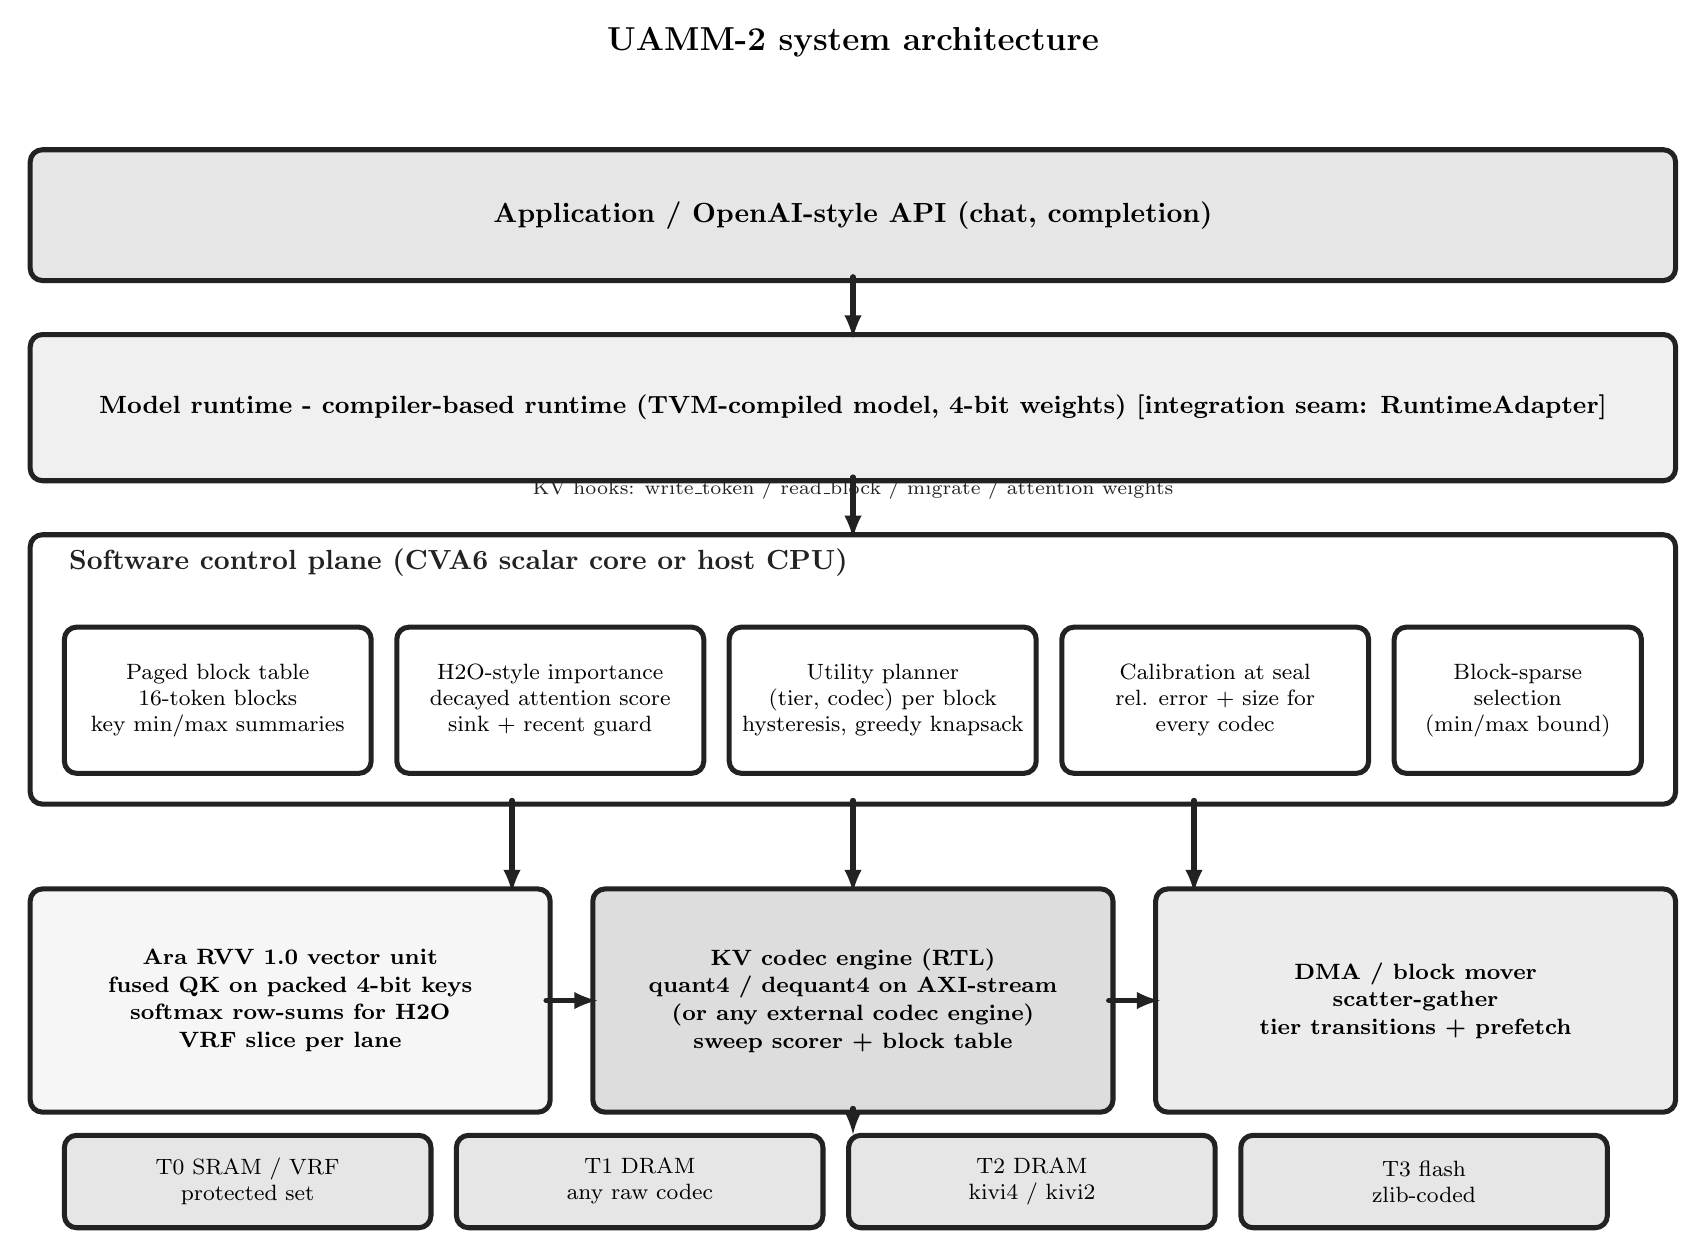
\begin{tikzpicture}[line cap=round,line join=round]
\draw[rounded corners=4.4pt,line width=1.82pt,draw={rgb,255:red,34;green,34;blue,34},fill={rgb,255:red,230;green,230;blue,230}] (0.149in,4.755in) rectangle (8.376in,5.409in);
\draw[rounded corners=4.4pt,line width=1.82pt,draw={rgb,255:red,34;green,34;blue,34},fill={rgb,255:red,240;green,240;blue,240}] (0.149in,3.754in) rectangle (8.376in,4.485in);
\draw[-latex,line width=1.82pt,draw={rgb,255:red,34;green,34;blue,34}] (4.263in,4.774in) -- (4.263in,4.466in);
\draw[-latex,line width=1.82pt,draw={rgb,255:red,34;green,34;blue,34}] (4.263in,3.773in) -- (4.263in,3.465in);
\draw[rounded corners=4.4pt,line width=1.82pt,draw={rgb,255:red,34;green,34;blue,34},fill={rgb,255:red,255;green,255;blue,255}] (0.149in,2.137in) rectangle (8.376in,3.484in);
\draw[rounded corners=4.4pt,line width=1.82pt,draw={rgb,255:red,34;green,34;blue,34},fill={rgb,255:red,255;green,255;blue,255}] (0.320in,2.291in) rectangle (1.854in,3.022in);
\draw[rounded corners=4.4pt,line width=1.82pt,draw={rgb,255:red,34;green,34;blue,34},fill={rgb,255:red,255;green,255;blue,255}] (1.982in,2.291in) rectangle (3.517in,3.022in);
\draw[rounded corners=4.4pt,line width=1.82pt,draw={rgb,255:red,34;green,34;blue,34},fill={rgb,255:red,255;green,255;blue,255}] (3.644in,2.291in) rectangle (5.179in,3.022in);
\draw[rounded corners=4.4pt,line width=1.82pt,draw={rgb,255:red,34;green,34;blue,34},fill={rgb,255:red,255;green,255;blue,255}] (5.307in,2.291in) rectangle (6.841in,3.022in);
\draw[rounded corners=4.4pt,line width=1.82pt,draw={rgb,255:red,34;green,34;blue,34},fill={rgb,255:red,255;green,255;blue,255}] (6.969in,2.291in) rectangle (8.205in,3.022in);
\draw[-latex,line width=1.82pt,draw={rgb,255:red,34;green,34;blue,34}] (2.558in,2.156in) -- (2.558in,1.694in);
\draw[-latex,line width=1.82pt,draw={rgb,255:red,34;green,34;blue,34}] (4.263in,2.156in) -- (4.263in,1.694in);
\draw[-latex,line width=1.82pt,draw={rgb,255:red,34;green,34;blue,34}] (5.968in,2.156in) -- (5.968in,1.694in);
\draw[rounded corners=4.4pt,line width=1.82pt,draw={rgb,255:red,34;green,34;blue,34},fill={rgb,255:red,246;green,246;blue,246}] (0.149in,0.597in) rectangle (2.749in,1.713in);
\draw[rounded corners=4.4pt,line width=1.82pt,draw={rgb,255:red,34;green,34;blue,34},fill={rgb,255:red,221;green,221;blue,221}] (2.962in,0.597in) rectangle (5.563in,1.713in);
\draw[rounded corners=4.4pt,line width=1.82pt,draw={rgb,255:red,34;green,34;blue,34},fill={rgb,255:red,236;green,236;blue,236}] (5.776in,0.597in) rectangle (8.376in,1.713in);
\draw[-latex,line width=1.82pt,draw={rgb,255:red,34;green,34;blue,34}] (2.728in,1.155in) -- (2.984in,1.155in);
\draw[-latex,line width=1.82pt,draw={rgb,255:red,34;green,34;blue,34}] (5.541in,1.155in) -- (5.797in,1.155in);
\draw[rounded corners=4.4pt,line width=1.82pt,draw={rgb,255:red,34;green,34;blue,34},fill={rgb,255:red,230;green,230;blue,230}] (0.320in,0.019in) rectangle (2.153in,0.481in);
\draw[rounded corners=4.4pt,line width=1.82pt,draw={rgb,255:red,34;green,34;blue,34},fill={rgb,255:red,230;green,230;blue,230}] (2.280in,0.019in) rectangle (4.113in,0.481in);
\draw[rounded corners=4.4pt,line width=1.82pt,draw={rgb,255:red,34;green,34;blue,34},fill={rgb,255:red,230;green,230;blue,230}] (4.241in,0.019in) rectangle (6.074in,0.481in);
\draw[rounded corners=4.4pt,line width=1.82pt,draw={rgb,255:red,34;green,34;blue,34},fill={rgb,255:red,230;green,230;blue,230}] (6.202in,0.019in) rectangle (8.035in,0.481in);
\draw[-latex,line width=1.82pt,draw={rgb,255:red,34;green,34;blue,34}] (4.263in,0.616in) -- (4.263in,0.485in);
\node[align=center,text={rgb,255:red,0;green,0;blue,0},font=\fontsize{10.0pt}{11.8pt}\selectfont\bfseries,inner sep=0pt] at (4.263in,5.082in) {Application / OpenAI-style API   (chat, completion)};
\node[align=center,text={rgb,255:red,0;green,0;blue,0},font=\fontsize{9.5pt}{11.2pt}\selectfont\bfseries,inner sep=0pt] at (4.263in,4.120in) {Model runtime  -  compiler-based runtime (TVM-compiled model, 4-bit weights)   [integration seam: RuntimeAdapter]};
\node[align=center,text={rgb,255:red,34;green,34;blue,34},font=\fontsize{7.5pt}{8.8pt}\selectfont,inner sep=0pt] at (4.263in,3.711in) {KV hooks: write\_token / read\_block / migrate / attention weights};
\node[anchor=south west,align=left,text={rgb,255:red,34;green,34;blue,34},font=\fontsize{10.0pt}{11.8pt}\selectfont\bfseries,inner sep=0pt] at (0.341in,3.272in) {Software control plane (CVA6 scalar core or host CPU)};
\node[align=center,text={rgb,255:red,0;green,0;blue,0},font=\fontsize{8.0pt}{9.4pt}\selectfont,inner sep=0pt] at (1.087in,2.656in) {Paged block table \\ 16-token blocks \\ key min/max summaries};
\node[align=center,text={rgb,255:red,0;green,0;blue,0},font=\fontsize{8.0pt}{9.4pt}\selectfont,inner sep=0pt] at (2.749in,2.656in) {H2O-style importance \\ decayed attention score \\ sink + recent guard};
\node[align=center,text={rgb,255:red,0;green,0;blue,0},font=\fontsize{8.0pt}{9.4pt}\selectfont,inner sep=0pt] at (4.412in,2.656in) {Utility planner \\ (tier, codec) per block \\ hysteresis, greedy knapsack};
\node[align=center,text={rgb,255:red,0;green,0;blue,0},font=\fontsize{8.0pt}{9.4pt}\selectfont,inner sep=0pt] at (6.074in,2.656in) {Calibration at seal \\ rel. error + size for \\ every codec};
\node[align=center,text={rgb,255:red,0;green,0;blue,0},font=\fontsize{8.0pt}{9.4pt}\selectfont,inner sep=0pt] at (7.587in,2.656in) {Block-sparse \\ selection \\ (min/max bound)};
\node[align=center,text={rgb,255:red,0;green,0;blue,0},font=\fontsize{8.5pt}{10.0pt}\selectfont\bfseries,inner sep=0pt] at (1.449in,1.155in) {Ara RVV 1.0 vector unit \\ fused QK on packed 4-bit keys \\ softmax row-sums for H2O \\ VRF slice per lane};
\node[align=center,text={rgb,255:red,0;green,0;blue,0},font=\fontsize{8.5pt}{10.0pt}\selectfont\bfseries,inner sep=0pt] at (4.263in,1.155in) {KV codec engine (RTL) \\ quant4 / dequant4 on AXI-stream \\ (or any external codec engine) \\ sweep scorer + block table};
\node[align=center,text={rgb,255:red,0;green,0;blue,0},font=\fontsize{8.5pt}{10.0pt}\selectfont\bfseries,inner sep=0pt] at (7.076in,1.155in) {DMA / block mover \\ scatter-gather \\ tier transitions + prefetch};
\node[align=center,text={rgb,255:red,0;green,0;blue,0},font=\fontsize{8.0pt}{9.4pt}\selectfont,inner sep=0pt] at (1.236in,0.250in) {T0  SRAM / VRF \\ protected set};
\node[align=center,text={rgb,255:red,0;green,0;blue,0},font=\fontsize{8.0pt}{9.4pt}\selectfont,inner sep=0pt] at (3.197in,0.250in) {T1  DRAM \\ any raw codec};
\node[align=center,text={rgb,255:red,0;green,0;blue,0},font=\fontsize{8.0pt}{9.4pt}\selectfont,inner sep=0pt] at (5.158in,0.250in) {T2  DRAM \\ kivi4 / kivi2};
\node[align=center,text={rgb,255:red,0;green,0;blue,0},font=\fontsize{8.0pt}{9.4pt}\selectfont,inner sep=0pt] at (7.118in,0.250in) {T3  flash \\ zlib-coded};
\node[anchor=south,align=center,text={rgb,255:red,0;green,0;blue,0},font=\fontsize{12.0pt}{14.2pt}\selectfont\bfseries,inner sep=0pt] at (4.263in,5.869in) {UAMM-2 system architecture};
\end{tikzpicture}
